\section{Theorie}
\label{sec:Theorie}

\subsection{Röntgenemissionsspektrum}
\label{sec:Theorie_emission}

Zur Erzeugung von Röntgenstrahlung werden in einer evakuierten Röhre durch eine
Glühkathode Elektronen freigesetzt. Diese werden durch eine sehr hohe Spannung zu
einer Anode hin stark beschleunigt. Beim Auftreffen der Elektronen auf die Anode
entsteht Röntgenstrahlung. Diese besteht aus der kontinuierlichen Bremsstrahlung
und der für das Material der Anode spezifischen und diskreten charakteristischen
Strahlung.

Das Bremsspektrum, das in Abbildung \ref{fig:bremsspektrum} skizziert ist, entsteht
durch das Abbremsen der Elektronen auf der Anode durch Coulombwechselwirkung. Dabei
wird ein Photon ausgesandt, das genau die Energie besitzt, die das Elektron durch
diesen Abbremsvorgang verliert. Das Elektron muss dabei nicht zwangsläufig völlständig
abgebremst werden, gibt also nicht in jedem Fall seine gesamte Energie ab. Aufgrunddessen
ist das Spektrum kontinuierlich. Das Spektrum hat jedoch eine untere Grenze $\lambda_{\symup{min}}$
für die Wellenlänge. Diese folgt dem Zusammenhang
\begin{equation}
  \lambda_{\symup{min}}=\frac{hc}{e_0 U} \,.
  \label{eqn:lambdamin}
\end{equation}
Dabei ist $h=6{,}626 \cdot 10^{-34} \,$Js das Planck'sche Wirkungsquantum,
$e_0=1{,}602 \cdot 10^{-19}\,$C die Elementarladung, $c$ die Lichtgeschwindigkeit
und $U$ die beschleunigende Spannung.
Die Photonen mit dieser Wellenlänge besitzen die gesamte kinetische Energie eines
Elektrons nun in Form von Stahlungsenergie.

\begin{figure}
  \centering
  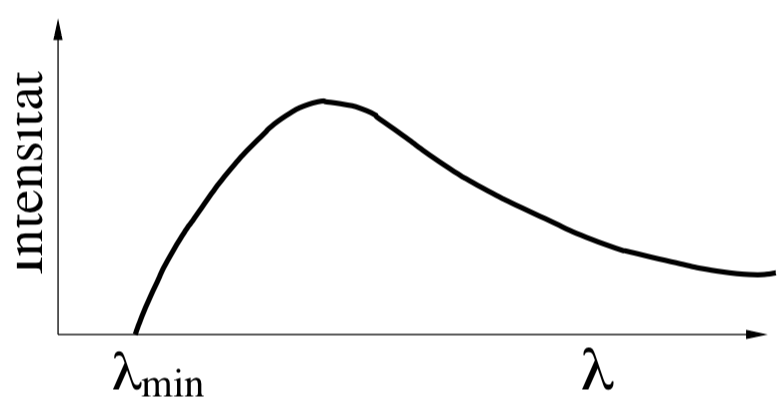
\includegraphics[height=4cm]{data/bremsspektrum.png}
  \caption{Skizze des kontinuierlichen Bremsspektrums \cite{Versuchsanleitung}.}
  \label{fig:bremsspektrum}
\end{figure}

Die charakteristische Stahlung entsteht dadurch, dass die hochenergetischen Elektronen
die Atome der Anode ionisieren, sodass in einer inneren Schale eine Leerstelle entsteht.
In diese Leerstelle kann nun ein Elektron von einer höheren Schale fallen. Da die
Energieniveaus auf den Schalen jedoch nicht identisch sind, wird bei diesem Vorgang
ein Photon ausgesandt, dass als Energie die Energiedifferenz der beiden Schalen besitzt:
\begin{equation}
  hf=E_{\symup{m}}-E_{\symup{n}} \,.
\end{equation}
Diese Energiedifferenzen sind charakteristisch für das Anodenmaterial.

In einem Atom mit mehreren Elektronen wird die Kernladung durch die Elektronen
abgeschirmt. Damit wird die Coulomb-Kraft auf ein Elektron auf der n-ten Schale auf
\begin{equation}
  E_{\symup{n}}=-R_{\symup{\infty}} z_{\symup{eff}}^2 \cdot \frac{1}{n^2}
  \label{eqn:bindungsenergie}
\end{equation}
reduziert. Dabei ist $R_{\symup{\infty}}=13.6\,$eV die Rydbergenergie und
$z_{\symup{eff}}=z-\sigma$ die effektive Kernladung, wobei $\sigma$ die
Abschirmkonstante ist.

%Jede charakteristische Linie besteht aus mehreren eng beieinanderliegenden Linien.
%Dies nennt man auch die Feinstruktur der charakteristischen Strahlung. Diese tritt auf,
%da die äußeren Elektronen aufgrund von Spins und Bahndrehimpulsen leicht unterschiedliche
%Bindungsenergien besitzen. Diese Bindungsenergie beschreibt die Sommerfeld'sche
%Feinstrukturformel:

%$R_{\symup{\infty}}$ ist hier erneut die Rydbergenergie und $z_{\symup{eff}}$ erneut
%die effektive Kernladungszahl. $\alpha$ ist die Sommerfeld'sche Konstante, $n$
%die Hauptquantenzahl und $j$ der Bahndrehimpuls des Elektrons.

\subsection{Röntgenabsorptionsspektrum}
\label{sec:Theorie_absorption}

Trifft Röntgenstrahlung auf Materie, so wird sie durch die Materie abgebremst und
abgelgenkt. Die bei den im Versuch auftretenden Energien dominant auftretenden
Prozesse sind der Photoeffekt und der Compton-Effekt.
Beim Compton Effekt werden die auf den Absorber treffenden Photonen abgelenkt.
Diese Ablenkung ist umso schwächer, je größer die Energie der Photonen ist. Daher
fällt der Absorptionskoeffizient mit steigender Photonenergie.
Beim Photoeffekt wird ein Röntgenquant von einem Elektron im Absorbermaterial absorbiert,
wodurch das Elektron auf eine andere Schale gehoben wird. Ist die Photonenenergie der
Röntgenstrahlung gerade so groß, dass dies möglich ist, kommt es daher zu einem
Anstieg der Absorption.
Eine Skizze des durch die beiden zuvor erläuterten Effekte entstehenden Absorptionsspektrums
ist in Abbildung \ref{fig:absorption} zu sehen.

\begin{figure}
  \centering
  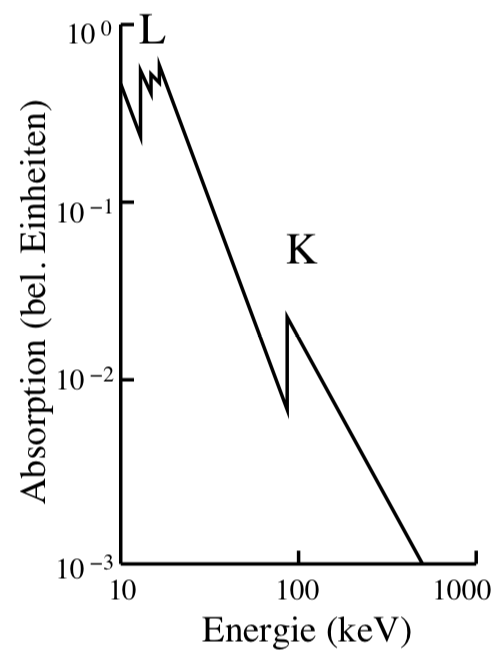
\includegraphics[height=4cm]{data/absorption.png}
  \caption{Skizze des Absorptionsspektrums \cite{Versuchsanleitung}.}
  \label{fig:absorption}
\end{figure}

Im Verlauf zeigen sich klare Kanten. Diese erhalten eine Bezeichnung durch die
Schale, aus der die Elektronen stammen, die nun die Röntgenquanten absorbieren.
Auch bei den Aborptionskanten ist eine Feinstruktur erkennbar, die sich mithilfe
der Sommerfeld'schen Freinstrukturformel
\begin{equation}
  E_{\symup{n,j}}=-R_{\symup{\infty}}\Biggl(z_{\symup{eff,1}}^2\cdot \frac{1}{n^2} +
   \alpha^2 z_{\symup{eff,2}}^4\cdot \frac{1}{n^3}\Biggl(\frac{1}{j+\frac{1}{2}} -
   \frac{3}{4n}\Biggr)\Biggr) \,.
   \label{eqn:sommerfeld}
\end{equation}
annähern lassen. Dabei Bezeichnet $E$ die Bindungsenergie eines Elektrons, $\alpha$ die Sommerfeld'sche
Feinstrukturkonstante, $n$ die Hauptquantenzahl und $j$ der Gesamtdrehimpuls des
Elektrons. $R_{\symup{\infty}}$ ist hier erneut die Rydbergenergie und $z_{\symup{eff}}$ erneut
die effektive Kernladungszahl.

Für die Bestimmung der Abschirmkonstante $\sigma_{\symup{L}}$ aus der L-Kante besteht ein
sehr komplexer Zusammenhang, der durch die Bestimmung der Energiedifferenz zweier
L-Kanten angenähert werden kann. Es ergibt sich für die im Versuch zu bestimmende
Abschirmkonstante
\begin{equation}
  \sigma_{\symup{L}}=Z-\left(\frac{4}{\alpha} \sqrt{\frac{\Delta E_{\symup{L}}}{R_{\symup{\infty}}}}
  -\frac{5\Delta E_{\symup{L}}}{R_{\symup{\infty}}}\right)^{1/2}
  \left(1+\frac{19}{32}\alpha^2 \frac{\Delta E_{\symup{L}}}{R_{\symup{\infty}}}\right)^{1/2} \,.
  \label{eqn:naeherung}
\end{equation}
Die experientelle Bestimmung der Energie ist mithilfe der Bragg'schen Reflexion
möglich. Dabei wird ein Kristall mit Röntgenlicht bestrahlt. Dabei wird das Licht
am Kristall gebeugt und es entstehen Interferenzen. Beim sogenannten Glanzwinkel
entsteht Konstruktive Interferenz. Die Bragg Bedingung
\begin{equation}
  2 d \sin(\theta)= n \lambda
  \label{eqn:bragg}
\end{equation}
folgt aus trigonometrischen Beziehungen am Kristall und liefert einen Zusammenhang
zwischen Wellenlänge und Winkel. Dabei ist $d$ der Netzebendenabstand der Gitterebenen
des Kristalls, $\theta$ der Winkel, den der Kristall mit der Horizontalen einschließt,
n die Beugungsordnung und $\lambda$ die Wellenlänge des Lichts.  Die Energie der
Röntgenphotonen folgt demnach dem Zusammenhang
\begin{equation}
  E=\frac{h c}{2 d \sin(\theta)} \,.
  \label{eqn:winkel}
\end{equation}


\subsection{Vorbereitende Rechnungen für die Bestimmung der K- und L-Kanten}
\label{subsec:K_L_Kanten}

Zur Vorbereitung der Messung werden für die zu verwendenden Elemente bereits
die Ordnungszahl und die Energie für die K-Kante aus \cite{xraydata} entnommen und
daraus der Winkel $\theta_{\symup{K}}$, unter dem die K-Kante zu messen sein wird,
nach Gleichung \eqref{eqn:winkel}, sowie die Abschirmkonstante $\sigma_{\symup{K}}$
für die K-Kante mithilfe von Gleichung \eqref{eqn:bindungsenergie} berechnet.
Die entnommenen Energien werden hierbei auf zwei Nachkommastellen gerundet.
Es ergeben sich die in Tabelle \ref{tab:theoriewerte} dargestellten Werte.

\begin{table}
	\begin{center}
    \caption{Theoretisch berechnete Werte für die Winkel und Abschirmkonstanten
    für die K-Kanten der zu verwendenden Elemente.}
    \label{tab:theoriewerte}
		\begin{tabular}{ccccc}
		\toprule
			& {$Z$} & {$E_{\symup{lit, K}}/$KeV} & {$\theta_{\symup{lit, K}}$} & {$\sigma_{\symup{K}}$}\\
			\midrule
			Zn & 30  & 9,67  &  18,56   &  3,33  \\
      Br &  35  & 13,48 &  13,20  &  3,52 \\
      Sr &  38  & 16,12 &  11,01  &  3,57 \\
      Zr &  40  & 18,01 &  9,84   &  3,61 \\
		\bottomrule
		\end{tabular}
	\end{center}
\end{table}

Für die L-Kanten von Gold werden Ebenfalls die Energien aus \cite{xraydata} entnommen
und analog gerechnet. Es ergeben sich die in Tabelle \ref{tab:goldtheo} dargestellten
Werte.

\begin{table}
	\begin{center}
    \caption{Theoretisch berechnete Werte für den Winkel und Abschirmkonstanten
    für die L-Kanten von Gold.}
    \label{tab:goldtheo}
		\begin{tabular}{ccc}
		\toprule
			 & {$E_{\symup{lit}}/$KeV} & {$\theta_{\symup{lit}}$}\\
			\midrule
			L1  &  14,36  & 12,39  \\
      L2  &  13,74  & 12,96  \\
      L3  &  11,93  & 14,96  \\
		\bottomrule
		\end{tabular}
	\end{center}
\end{table}
Für die Abschirmkonstante ergibt sich mithilfe von Gleichung \eqref{eqn:naeherung}
ein Näherungswert von $\sigma_{\symup{L}}=3{,}62$.

%Hier vielleicht noch das mit den K-Linien des Emissionsspektrums und die Rechnung
%für Gold?
